\documentclass{article}
\usepackage{amsthm}
\usepackage{graphicx}
\usepackage{ctex}
\usepackage{amsmath}
\usepackage{amssymb} % 添加 amssymb 以支持更多符号
\usepackage{amsfonts}
\usepackage{tikz}
\usepackage{cancel}
\usepackage{listings}
\usetikzlibrary{arrows.meta} % 箭头样式
\title{离散数学作业\_4}
\author{李云浩 241880324}
\date{\today}
\lstset{
    language=C++, % 设置语言
    basicstyle=\ttfamily\small, % 基本字体
    numbers=left, % 行号在左侧
    numberstyle=\tiny\color{gray}, % 行号样式
    frame=single, % 边框
    captionpos=b, % 标题位置(底部)
    breaklines=true, % 自动换行
    keywordstyle=\color{blue}, % 关键字颜色
    commentstyle=\color{ForestGreen}, % 注释颜色
    stringstyle=\color{red}, % 字符串颜色
    tabsize=4 % 制表符替换为4空格
}
\begin{document}
\maketitle
\section{4.1}
\subsection{T16}
对于$A_1 \times A_2 \times A_3 = \{(a, b, c) | a \in A_1 \land b \in A_2 \land c \in A_3\}$,
因此可能元素的个数为:$C_{n_1}^1 \times C_{n_2}^1 \times C_{n_3}^1 = n_1 \times n_2 \times n_3$.证毕。
\subsection{T18}
投影(选择$\ $雇员[部门 = 人力资源部 $\lor$ 公共关系])
\subsection{T24}
不是,划分要求所有划分块的并集应该为原集合。但是因为$0 \in Z, 0 \notin A_1 \cup A_2$,
因此$\{A_1, A_2\}$不是$Z$的一个划分。
\subsection{T30}
(a) $A_1 = \{x | x \in B \land x \mid 2\}, A_2 = \{x | x \in B \land x \nmid 2\}$。
$\{A_1, A_2\}$是$B$的一个划分。

(b) $A_1 = \{x | x \in B \land x \mid 9\}, A_2 = \{x | x \in B \land x \nmid 9 \land x \mid 6\},
A_3 = \{x | x \in B \land x \nmid 9 \land x \nmid 6 \land x \mid 3\}$。
$\{A_1, A_2, A_3\}$是$B$的一个划分。
\subsection{T31}
$\{\{1, 2, 3\}\}, \{\{1\}, \{2, 3\}\}, \{\{2\}, \{1, 3\}\}, \{\{3\}, \{1, 2\}\}, 
\{\{1\}, \{2\}, \{3\}\}$
\subsection{T33}
由已知有:$S(3, 2) = S(2, 1) + 2S(2, 2) = 3$,在31题中,两个子集的划分数也为3,
符合预期。
\subsection{T34}
由已知有:$S(4, 2) = S(3, 1) + 2S(3, 2) = 1 + 2 \times 3 = 7$。
\subsection{T35}
$S(4, 3) = S(3, 2) + 3S(3 , 3) = 3 + 3 \times 1 = 6$.
\subsection{T36}
$S(5 ,2) = S(4, 1) + 2S(4, 2) = 1 + 2 \times \{S(3, 1) + 2S(3, 2)\} = 1 + 2 \times \{1 + 2 \times 3\} = 15$
\subsection{T37}
设$(a, b) \in A \times (B \cup C)$,有:
\begin{align*}
    a(A \times (B \cup C))b &= a(A \times (Bb \cup Cb))\\
    &= aA \times (Bb \cup Cb)\\
    &= aA \times Bb \cup aA \times Cb\\
    &= a(A \times B)b \cup a(A \times C)b\\
    &= a((A \times B) \cup (A \times C))b\\
\end{align*}
因此,$A\times (B \cup C) = (A \times B) \cup (A \times C)$。
\subsection{T38}
由已知有:$B \cap C = \{7\}, A \times B = \{(1, 2), (1, 5), (1, 7), (2, 2), (2, 5), (2, 7), 
(4, 2), (4, 5), (4, 7)\}\\ 
A \times C = \{(1, 1), (1, 3), (1, 7), (2, 1), (2, 3), (2, 7), (4, 1), (4 ,3), (4, 7)\}$\\
因此:$A \times (B \cap C) = \{(1, 7), (2, 7), (4, 7)\}, (A \times B) \cap (A \times C) = \{(1, 7), (2, 7), (4, 7)\}$.
可知:$A \times (B \cap C) = (A \times B) \cap (A \times C)$

设$(a, b) \in A \times (B \cap C)$,有:
\begin{align*}
    a(A \times (B \cap C))b &= a(A \times (Bb \cap Cb))\\
    &= aA \times (Bb \cap Cb)\\
    &= aA \times Bb \cap aA \times Cb\\
    &= a(A \times B)b \cap a(A \times C)b\\
    &= a((A \times B) \cap (A \times C))b\\
\end{align*}
因此$A \times (B \cap C) = (A \times B) \cap (A \times C)$。
\subsection{T39}
将B的划分中的各个集合中的独属于B的元素删去,若删去后为空集则直接将该集合去掉,否则则保留删除后的集合。
那么新子集组成的集合便是A的一个划分。

下面验证该过程:1.删去了所有的空集,因此划分块不为空。2.新的划分块是在B的划分块中删元素,原来不相交,
删除元素后也不会相交。3.因为只删去了独属于B的元素,因此新的划分包含A的所有元素。检验完毕。
\subsection{T40}
1. 证明划分块不为空,因为$A_i \neq \varnothing, B_j \neq \varnothing$,因此$A_i \times B_j \neq \varnothing$。\\
2. 证明划分块不相交,因为$\{A_1, A_2, \dots, A_k\}$是A的一个划分,因此对于$\forall i, j, i\neq j, \forall x \in A_i \rightarrow x \notin A_j$。
同理,B也一样。因此对于$\forall (x, y) \in A_i \times B_j, \rightarrow \forall m \neq i\forall n \neq j, (x \notin A_m \land y \notin B_n \rightarrow (x, y) \notin A_m \times B_n)$。
3. 证明划分块的并集为$A \times B$。由题目可知,每一个$A_i$都与$B_j$计算笛卡尔积,且$A_i,B_j$分别包含A,B中的所有元素。
因此所有$A_i \times B_j$的并集为$A \times B$。
\section{4.2}
\subsection{T20}
1. 证明:$\forall a \forall b(a, b \in A \land a \neq b \land R(a) \cap R(b) = \{\ \}) \subseteq R(A_1 \cap A_2) = R(A_1) \cap R(A_2)$\\
因为$R(a) \cap R(b) = \{\ \}$。\\
如果$A_1 \cap A_2 = \varnothing$,那么$R(A_1 \cap A_2) = R(\varnothing) = \{\ \}$。
由于$A_1$和$A_2$之中没有重复元素,因此对于任意$A_1, A_2$中的元素$a, b$,$R(a) \cap R(b) = \{\ \}$,所以$R(A_1) \cap R(A_2) = \{\ \}$。\\
如果$A_1 \cap A_2 = A_3$,那么$R(A_1 \cap A_2) = R(A_3)$,$R(A_1) \cap R(A_2) = (R(A_1 - A_2) \cup R(A_3)) \cap R(A_2) = 
(R(A_1 - A_2) \cap R(A_2)) \cup (R(A_3) \cap R(A_2)) = R(A_3)$,所以$R(A_1 \cap A_2) = R(A_1) \cap R(A_2)$。

2. 证明:$R(A_1 \cap A_2) = R(A_1) \cap R(A_2) \subseteq \forall a \forall b(a, b \in A \land a \neq b \land R(a) \cap R(b) = \{\ \})$\\
反证法:假设$R(a) \cap R(b) \neq \{\ \}$。那么取子集$A_1, A_2$分别为$\{a\}, \{b\}$。$R(A_1 \cap A_2) = R(\varnothing) = \{\ \}$。
但是$R(a) \cap R(b) \neq \{\ \}$。因此$R(A_1 \cap A_2) \neq R(A_1) \cap R(A_2)$。

因此
$R(A_1 \cap A_2) = R(A_1) \cap R(A_2) \subseteq \forall a \forall b(a, b \in A \land a \neq b \land R(a) \cap R(b) = \{\ \})$
\subsection{T25}
$
\begin{pmatrix}
    0 & 1 & 0 & 0 & 0\\
    0 & 1 & 1 & 0 & 0\\
    0 & 0 & 0 & 1 & 0\\
    0 & 0 & 0 & 1 & 0\\
    1 & 0 & 0 & 1 & 0
\end{pmatrix}
$
\subsection{T26}
$
\begin{pmatrix}
    0 & 1 & 1 & 1 & 0\\
    0 & 1 & 1 & 0 & 0\\
    0 & 0 & 0 & 0 & 0\\
    1 & 0 & 0 & 1 & 1\\
    0 & 0 & 0 & 0 & 0
\end{pmatrix}
$
\subsection{T28}
\begin{tabular}{c|c|c}
    顶点 & 入度 & 出度\\
    \hline
    1 & 1 & 3\\
    2 & 2 & 2\\
    3 & 2 & 0\\
    4 & 2 & 3\\
    5 & 1 & 0
\end{tabular}
\subsection{T32}
只保留B中元素所代表的行和列。
\subsection{T34}
设$M_R = [m_{ij}]_{n \times n}$\\
(a) $R(a_k) = \{m_{ki} | m_{ki} = 1 \land 0 \leq i \leq n\}$\\
(b) $R(\{a_l, a_j, a_n\}) = \{m_{ij} | m_{ij} = 1 \land (i = l \lor i = j \lor i = n) \land m_{ij} = 1\}$
\subsection{T36}
因为$|\{1, 2, 3\}| = 3, |\{a, b\}| = 2$,所以S中关系的数量为$2^{3 \times 2} = 2^6 = 64$ 
\section{4.3}
\subsection{T18}
\begin{align*}
    M_{R \cup S} &= \{m_{ij} | i (R \cup S) j\}\\
    &= \{m_{ij} | iRj \lor iSj\}\\
    &= \{m_{ij} | iRj\} \lor \{m_{ij} | iSj\}\\
    &= M_R \lor M_S
\end{align*}
\subsection{T19}
因为$R^*$的定义是$x = y$或$x R^{\infty} y$。因此$M_{R^*} = \{m_{ij} | i = j\} \lor \{m_{ij} | x R^{\infty} y\}$
所以$M_{R^*} = M_{R^{\infty}} \lor I_n$
\subsection{T20}
$\pi_2 \circ \pi_1 = 1, 2, 4, 3, 5, 6, 4$
\subsection{T21}
$\pi_2 \circ \pi_1 = 1, 7, 5, 6, 7, 4, 3$
\subsection{T27}
$M_R = 
\begin{bmatrix}
    1 & 1 & 1 & 1\\
    0 & 0 & 1 & 0\\
    0 & 1 & 0 & 0\\
    0 & 1 & 1 & 1
\end{bmatrix}
,\quad M_R \cdot M_R = 
\begin{bmatrix}
    1 & 3 & 3 & 2\\
    0 & 1 & 0 & 0\\
    0 & 0 & 1 & 0\\
    0 & 2 & 2 & 1
\end{bmatrix}$
其中$m_{ij}$表示从i 到 j且长度为2的路线的数目。
\subsection{T28}
$(M_R)^3 = 
\begin{bmatrix}
    9 & 6 & 6 & 3\\
    0 & 0 & 1 & 0\\
    0 & 1 & 0 & 0\\
    0 & 3 & 3 & 1
\end{bmatrix}$
显然,$(M_R)^3$的$m_{ij}$不表示从i 到 j且长度为3的路线的数目。
\subsection{T30}
(a)定理2 先说明了P(2)为真,在此基础上以P(n)为真作为前提条件,从而推导出P(n + 1)为真,最后便可以
通过归纳得出结论,即:对于整数$n \leq 2,P(n)$成立。
(b)以P(n)成立作为前提条件,并把P(n)翻译为自然语言,通过自然语言建立P(n)与P(n + 1)的联系。
\subsection{T31}
设一共有n个顶点,且每个顶点的出度不为1。那么$\forall n \in Z, R^n$不为空,因为每个顶点皆有出度。
但由于只有n个顶点,但$R^{\infty}$存在,即存在一条无限长的路径,因此有向图中有环。因此可以得出,如果
在D中无任何环,那么至少有一个顶点的出度是0
\subsection{T32}
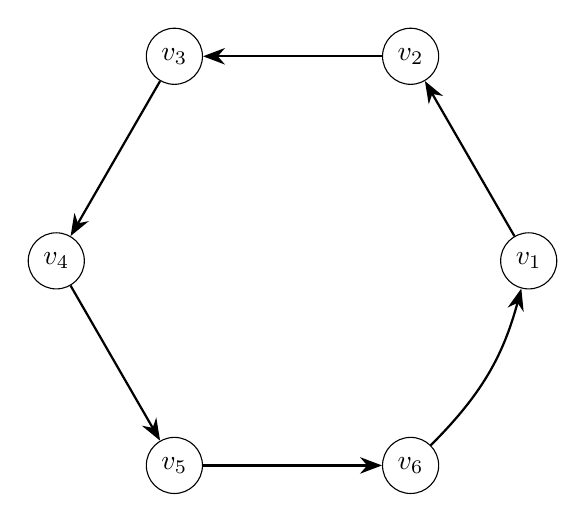
\begin{tikzpicture}[
    node distance=2cm,
    vertex/.style={circle, draw, minimum size=6mm},
    edge/.style={-{Stealth[scale=1.2]}, thick} % 定义箭头样式
]

% 绘制顶点
\foreach \i in {1,...,6} {
    \node[vertex] (v\i) at (60*\i-60:3cm) {$v_\i$};
}

% 绘制长度为6的道路:v1 -> v2 -> ... -> v6
\foreach \i [evaluate=\i as \j using int(\i+1)] in {1,...,5} {
    \draw[edge] (v\i) -- (v\j);
}

% 添加一条额外边(确保只有6条长度为1的道路)
\draw[edge, bend right=15] (v6) to (v1); % 例如:v6 -> v1

\end{tikzpicture}
\subsection{T33}
将有向图转换为关系矩阵,这样可以更加直观的看出。
\section{4.4}
\subsection{T14}
1.自反性:$\forall x \in A, |x - x| = 0 \leq 2$成立,因此$\forall x \in A \rightarrow (x, x)\in R$。满足自反性。\\
2.反自反性:由于满足自反性,因此不满足反自反性。\\
3.对称性:$\forall a, b\in A, |a - b| = |b - a|$,因此$\forall a, b \in A, (a, b)\in R \rightarrow (b, a) \in R$,满足对称性。\\
4.反对称性:反例:$(1, 2) \in R \land (2, 1) \in R \land 2 \neq 1$,因此不满足反对称性。\\
5.传递性:反例:$(0, 2) \in R \land (2, 4) \in R$,但是$(0, 4) \notin R$,因此不满足传递性。\\
\subsection{T16}
1.自反性:$\forall x \in A, x + x = 2x$,为2的倍数即偶数,因此满足自反性。\\
2.反自反性:由于满足自反性,因此不满足反自反性。\\
3.对称性:$\forall a, b \in A, a + b = b + a$。因此$\forall a, b \in A, (a, b) \in R \rightarrow (b, a) \in R$。\\
4.反对称性:反例:$(2, 4) \in R \land (4, 2) \in R \land 2 \neq 4$,因此不满足反对称性\\
5.传递性:如果$a + b$为偶数,那么a, b要么同为奇数,要么同为偶数。因此,对应奇偶性明确的数字$b$,如果$(a,b) \in R \land (b, c) \in R$,
那么$a, c$的奇偶性一定与$b$等同,因此$a, c$的奇偶性一致,因此$(a,c)\in R$。满足传递性。
\subsection{T18}
1.自反性:反例:$4 \in A, (4, 4) \notin R$,因此不满足自反性\\
2.反自反性:反例:$\sqrt2 \in A, (\sqrt2, \sqrt2) \in R$,因此不满足反自反性\\
3.对称性:因为$\forall a, b \in A, a^2 + b^2 = b^2 + a^2$,因此$\forall a, b \in A, (a,b)\in R \rightarrow (b,a) \in R$,
满足对称性\\
4.反对称性:取$a = 1, b = \sqrt3$,因为$(a, b) \in R \land (b, a) \in R \land a\neq b$,因此不满足反对称性。\\
5.传递性:反例:$(1, \sqrt3) \in R \land (\sqrt3, 1) \in R \land (1, 1)\notin R$,因此不满足传递性。
\subsection{T20}
1.自反性:$\forall (a, b) \in A$,因为$a = a$,所以有$(a, b)R (a, b)$满足自反性。\\
2.反自反性:由于满足自反性,因此不满足反自反性。\\
3.对称性:$\forall (a, b), (c, d) \in A$,如果$ a = c \rightarrow c = a$,因此$(a, b) R (c, d) \rightarrow a = c 
\rightarrow (c, d) R (a, b)$,因此满足对称性\\
4.反对称性:反例:$(1, 3) R (1, 4) \land (1, 4) R (1, 3) \land (1, 3) \neq (1, 4)$,因此不满足反对称性。\\
5.传递性:$\forall (a, b), (c, d), (e, f) \in A \land (a, b) R (c, d) \land (c, d) R (e, f)$,因此有:$a = c, c = e$,
因此$a = e \rightarrow (a, b) R (e, f)$,因此满足传递性。
\subsection{T22}
1.自反性:因为直线平行于自身,因此$\forall l_i \in A, l_i R l_i$,满足自反性。\\
2.反自反性:由于满足自反性,因此不满足反自反性。\\
3.对称性:因为$l_i \parallel l_j \rightarrow l_j \parallel l_i$,因此$\forall l_i, l_j \in A \land l_i R l_j \rightarrow
l_j R l_i$,因此满足对称性。\\
4.反对称性:反例:$l_1:y = x, l_2: y = x + 1$,因此$l_1 R l_2 \land l_1 \neq l_2$,因此不满足反对称性。\\
5.传递性:因为平行本身具有传递性,因此$\forall l_i, l_j, l_k \in A$,如果$l_i R l_j \land l_j R l_k \rightarrow l_i R l_k$,因此满足传递性
\subsection{T31}
因为集合$A$上的关系是反自反,因此其关系矩阵中的主对角线上全为0.那么证明该集合的关系具有反对称的性质可以转换为证明$\nexists a, b \in A, a R b \land b R a$。\\
下用反证法,不妨假设$\exists a, b \in A, a R b \land b R a$,
因为该关系具有传递性,$a R b \land b R a \rightarrow a R a$,与反自反的条件不符,因此假设不成立。
因此$\nexists a, b \in A, a R b \land b R a$,故该关系是反对称的,并且因为主对角线元素全为0,所以还是非对称的。
\subsection{T32}
反证法:假设$R^2$不满足传递性,则$\exists a, c, e \in A, a R c \land c R e \land a \cancel{R} e$。
因为$R^2$是由$R$复合运算得来的,因此$\exists b, d \in A, a R b, b R c, c R d, d R e$。因为$R$是传递的,
那么在$R$中一定还有$a R c \land c R e$,因此$R^2 = R \circ R$中会含有$a R e$,与假设不符,因此假设不成立。\\
故如果A上的关系R是传递的,那么$R^2$也是传递的。
\subsection{T33}
因为$R$是对称的,因此$\exists a, b \in A, aRb \land bRa$,又因为$R$是传递的,因此$aRb \land bRa \rightarrow aRa$,
因此$\exists a \in A, (a, a) \in R$,因此$R$不是非自反的。
\subsection{T34}
$\forall (a, c) \in R^2$,因为$R^2$是由$R$复合而成,因此$\exists b \in A, (a, b) \in R \land (b, c) \in R$,
又因为$R$是对称的,因此$(c, b) \in R \land (b, a) \in R$.又因为$R^2 = R \circ R$,因此$(c, a) \in R^2$。即
$\forall (a, c) \in R^2 \rightarrow (c, a) \in R^2$,因此$R^2$也是对称的。
\subsection{T35}
当n = 1 时,显然成立。当 n = 2时,已有上题证出。\\
不妨假设当$n = k$时,结论成立,即$R^k$是对称的,下证$R^{k + 1}$也是对称的。\\
$\forall (a, c) \in R^{k + 1}$,因为$R^{k + 1} = R^{k} \circ R$,因此$\exists b \in A, (a ,b) \in R^k \land (b, c) \in R$
因为$R$和$R^k$是对称的,因此$(b, a) \in R^k \land (c, b) \in R$。又因为$R^{k + 1} = R \circ R^k$,因此$(c, a) \in R^{K + 1}$。
即$\forall (a, c) \in R^{k + 1} \rightarrow (c, a) \in R^{k + 1}$,因此$R^{k + 1}$也是对称的。\\
根据数学归纳法得出:如果$A$上的关系$R$是对称的,那么$R^n$对于任意$n \geq 1$也是对称的。
\subsection{T36}
定义:差3关系,即两数之差为3的倍数。$R = \{(a, b) | (a - b) \mid 3\}$。\\
1.自反性:$\forall a \in Z^{+}, a - a = 0$,为3的倍数,因此$\forall a \in Z^{+}, a R a$。满足自反性。\\
2.对称性:$\forall a, b \in Z^{+}$,如果$(a, b) \in R$,即$(a - b) \mid 3$,即$\exists m \in Z, a - b = 3m$。
因此$b - a = -3m$,仍为3的倍数。因此$\forall a, b \in Z^{+} \land (a, b)\in R \rightarrow (b, a) \in R$,满足对称性。\\
3.传递性:$\forall a, b, c \in Z^{+}, a R b, b R c$,因此$\exists m, n\in Z, (a - b) = 3m, (b - c) = 3n$。
那么$a - c = a - b + (b - c) = 3m + 3n = 3(m + n)$,仍为3的倍数。所以$\forall a, b, c \in Z^{+} \land aRb \land bRc 
\rightarrow a R c$,满足传递性。
\subsection{T38}
(a) $R = \{(a, b), (b, c), (a, c)\}$\\
(b) $R = \{(a, a), (b, b), (c, c), (d, d), (a, b), (b, c)\}$
\subsection{T40}
1.充分性:R是传递的 $\rightarrow$ 对于所有$n \geq 1, R^n \subseteq R$。\\
利用数学归纳法:当$n = 2$时,因为$R^2 = R \circ R$,因此$\forall (a, c) \in R^2
\rightarrow \exists b \in A \land (a, b) \in R \land (b, c) \in R$。因为$R$具有传递性,
因此$(a, c) \in R$。即$\forall (a, c) \in R^2 \rightarrow (a, c) \in R$。即$R^2 \subseteq R$。\\
当$n \geq 2$时,不妨设$n = k - 1$时,有$R^{k - 1} \subseteq R$。下证$R^k \subseteq R$。\\
因为$R^k = R^{k - 1} \circ R$, $\forall (a, c) \in R^k \rightarrow \exists b \in A \land (a, b) \in R^{k - 1} \land (b, c) \in R$。
又因为$R^{k - 1} \subseteq R$,因此$(a, b) \in R \land (b, c) \in R$。因为$R$具有传递性,因此$(a, c) \in R$。
即$\forall (a, c) \in R^k \rightarrow (a, c) \in R$,因此$R^k \subseteq R$。证毕。

2.必要性:对于所有$n \geq 1, R^n \subseteq R \rightarrow $ R是传递的。\\
取$ n = 2$,有:$R^2 \subseteq R$。$\forall (a, b), (b, c) \in R$,因为$R^2 = R \circ R$。
因此$(a, c) \in R^2$。又因为$R^2 \subseteq R$,因此$(a, c) \in R$。即$\forall (a, b) , (b, c) \in R 
\rightarrow (a, c) \in R$。因此$R$是传递的,证毕。
\section{4.5}
\subsection{T19}
(a)1.自反性:$\forall (a, b) \in A, a^2 + b ^2 = a^2 + b^2$,因此$(a, b) R (a, b)$,满足自反性。\\
2.对称性:$\forall (a, b) \in A, a^2 + b^2 = b^2 + a^2$,因此$(a, b) R (b, a)$,满足对称性。\\
3.传递性:$\forall (a, b), (c, d), (e, f) \in A \land (a, b) R (c, d) \land (c, d) R (e, f)$。因此
$a^2 + b^2 = c^2 + d^2 = e^2 + f^2$,所以$a^2 + b^2 = e^2 + f^2$,即$(a, b) R (e, f)$。故$\forall
(a, b), (c, d), (e, f) \in A \land (a, b) R (c, d) \land (c, d) R (e, f) \rightarrow (a, b) R (e, f)$。
满足传递性。\\
因为关系R满足自反、对称、传递性,因此R是A上的一个等价关系。

(b)在每个等价类中,$a^2 + b^2 = c^2 + d^2$,可以理解为坐标到原点的距离相等,即圆。
因此$A / R$为以原点为圆心的无数个圆。
\subsection{T20}
因为等价关系具有对称性,因此只观察关系矩阵的右上角部分,有:$\{(a, a), (a, b), (a, c), (a, e),
(b, b), (b, c), (b, e), (c, c), (c, e), (d, d), (e, e)\} \subseteq R$,因此不难得出:
a与b, c, e等价,d与自身等价。因此$A / R = \{\{a, b, c, e\}, \{d\}\}$
\subsection{T22}
(a)1.自反性:$\forall (a, b) \in A, a + b = a + b$,因此$(a, b) R (a, b)$。满足自反性。\\
2.对称性:$\forall (a, b) \in A, a + b = b + a$,因此$(a, b) R (b, a)$。满足对称性。\\
3.传递性:$\forall (a, b), (c, d), (e, f) \in A \land (a, b) R (c, d) \land (c, d) R (e, f)$。因此:
$a + b = c + d = e + f$,有$(a, b) R (e, f)$。因此满足传递性。\\
因此R是一个等价关系。
(b)可以根据$a + b$的和来进行等价类划分。
$A / R = \{\{(1, 1)\}, \{(1, 2), (2, 1)\}, \{(1, 3), (3, 1), (2, 2)\}, \{(1, 4), (2, 3), (3, 2), (4, 1)\}, \\
\{(2, 4), (3, 3), (4, 2)\}, \{(3, 4), (4, 3)\}, \{(4, 4)\}\}$
\subsection{T23}
1.充分性:$R$是自反的和循环的 $\rightarrow$ $R$是一个等价关系。\\
证$R$是等价关系,即证$R$具有自反、对称、传递性。已知,$R$具有自反性。\\
对称性:$\forall (a, b) \in R$,因为自反性,所以$(a, a) \in R$,根据传递性可以得:$(a, a)\in R \land (a, b) \in R \rightarrow (b, a) \in R$。
即:$\forall (a, b) \in R \rightarrow (b, a) \in R$。因此$R$是对称的。\\
传递性:$\forall (a, b), (b, c) \in R$根据循环性,所以$(c, a) \in R$。又因为对称性,所以$(a, c) \in R$。因此$\forall (a, b), (b, c) \in R
\rightarrow (a, c) \in R$。

2.必要性:$R$是等价关系 $\rightarrow$ $R$是自反的和循环的。 \\
因为$R$是等价的,因此$R$一定是自反的。又因为$\forall (a, b), (b, c) \in R$,因为$R$是等价的,
因此$R$具有传递性,所以$(a, c) \in R$。又因为$R$具有传递性,所以$(c, a) \in R$。即$\forall (a, b), (b, c) \in R
\rightarrow (c, a) \in R$。因此$R$是循环的。
\subsection{T24}
1.自反性:$\forall x \in A$,因为$R_1, R_2$,具有自反性,所以$(x, x) \in R_1, (x, x) \in R_2$。因为$R_1 \cap R_2$即取$R_1, R_2$中的公共元素。
因此$(x, x) \in R_1 \cap R_2$。即:$\forall x \in A \rightarrow (x, x) \in R_1 \cap R_2$。满足自反性。\\
2.对称性:
\begin{align*}
    \forall (a, b) \in R_1 \cap R_2 &\Rightarrow (a, b) \in R_1 \land (a, b) \in R_2\\
    &\Rightarrow (b, a) \in R_1 \land (b, a) \in R_2\\
    &\Rightarrow (b, a) \in R_1 \cap R_2
\end{align*}因此$R_1 \cap R_2$满足对称性。\\
3.传递性:
\begin{align*}
    \forall (a, b), (b, c) \in R_1 \cap R_2 &\Rightarrow (a, b) \in R_1 \land (b, c) \in R_1 \land (a, b) \in R_2 \land (a, b) \in R_2\\
    &\Rightarrow (a, c) \in R_1 \land (a, c) \in R_2\\
    &\Rightarrow (a, c) \in R_1 \cap R_2
\end{align*}因此$R_1 \cap R_2$满足传递性。\\
综上所述,$R_1 \cap R_2$是$A$上的一个等价关系。
\subsection{T27}
因为R是模2同余关系,有$\forall x \in R(a)$,$x$与$a$的奇偶性相同。\\
情况1:$a, b$同奇偶性,因为$R(a) + R(b) = \{x | x = s + t, s \in R(a), t \in R(b)\}$,
且$s, t$的奇偶性也相同,因此$\forall x \in (R(a) + R(b))$一定为偶数。又因为$a, b$同奇偶性,因此$a + b$亦为偶数。
因此:$\forall x(x \in (R(a) + R(b)) \leftrightarrow x \in R(a + b))$。\\
情况2:$a, b$的奇偶性相反,因为$R(a) + R(b) = \{x | x = s + t, s \in R(a), t \in R(b)\}$,
且$s, t$的奇偶性也相同,因此$\forall x \in (R(a) + R(b))$一定为奇数。又因为$a, b$奇偶性相反,因此$a + b$亦为奇数。
因此:$\forall x(x \in (R(a) + R(b)) \leftrightarrow x \in R(a + b))$。\\
综上所述:对所有$a, b$,有$R(a) + R(b) = R(a + b)$。
\subsection{T28}
不妨设:$a = (m_a, n_a), b = (m_b, n_b)$.\\
因此$R(a) = \{(m_i, n_i) | n_i = n_a\}, R(b) = \{(m_j, n_j) | n_j = n_b\}$,
所以$R(a) + R(b) = \{(m_k, n_k) | m_k = m_i + m_j, n_k = n_i + n_j, (m_i, n_i) \in R(a), (m_j, n_j) \in R(b)\}
= \{(m_k, n_k) | n_k = n_a + n_b\}$。
因为$R(a + b) = \{(m_l, n_l) | n_l = n_a + n_b\}$。因此$(R(a) + R(b))$与$R(a+b)$的集合的定义相同,所以$R(a) + R(b) = R(a + b)$。
\subsection{T29}
因为$R((a, b)) = \{(m_i, n_i) | an_i = bm_i\}, R((a', b')) = \{(m_j, n_j) | a'n_j = b'm_j\},
R((a + a', b + b')) = \{(m_k, n_k) | (a + a')n_k = (b + b')m_k\}$。又因为$R((a, b)) + R((a', b'))
= \{(m_l, n_l) | (m_l, n_l) = (m_i, n_i) + (m_j, n_j), (m_i, n_i) \in R((a, b)), (m_j, n_j) \in R((a', b'))\}$。
要证$R((a, b)) + R((a', b')) = R((a + a', b + b'))$,即证$\forall (m_l, n_l) \in (R((a, b)) + R((a', b'))) \rightarrow
(a + a')n_l = (b + b')m_l$。因为$(a + a')(n_i + n_j) - (b + b')(m_i + m_j) = an_j + a'n_i - bm_j - b'm_i$。不一定为0。
因此等式不成立。\\
较容易举出反例:$(1, 2) R (2, 4), (1, 3) R (2, 6)$但是$(3, 7) \notin R((2, 5))$
\section{4.6}
\subsection{T2}
\begin{lstlisting}
    EDGE(i ,j){
        int ptr = VERT[i];
        while(NEXT[ptr] != 0){
            if(HEAD[ptr] == j){
                return T;
            }
            ptr = NEXT[ptr];
        }
        if(NEXT[ptr] == 0 && HEAD[ptr] == j) return T;
        else return F;
    }
\end{lstlisting}
\subsection{T3}
因为$R$一共有$P$条边,$N$个顶点。因此平均每个顶点的出度为$\frac{P}{N}$。对这$\frac{P}{N}$个出度进行排序,
如果要找的边为第$n$条,则需要$n$步,如果找的边不存在,那么则需要$\frac{P}{N}$步。
因此平均步数为:$\frac{1 + 2 + \dots + \frac{P}{N} + (N - \frac{P}{N})(\frac{P}{N})}{N} = \frac{(2N - \frac{P}{N} + 1)(\frac{P}{N})}{2N}$
\subsection{T4}
\begin{lstlisting}
    LOOK(NUM, NEXT, START, N, K){
        int ptr = START;
        while(NEXT[ptr] != 0){
            if(NUM[ptr] == K) return ptr;
            else ptr == NEXT[ptr];
        }
        if(NUM[ptr] != K) print("NOT FOUND");
        else return ptr;
    }
\end{lstlisting}
\subsection{T6}
$$
\begin{array}{|c|c|c|c|}
    VERT & TAIL & HEAD & NEXT\\
    \hline
    2 & 4 & 1 & 9\\
    4 & 1 & 1 & 3 \\
    7 & 1 & 2 & 5\\
    1 & 2 & 1 & 6\\
    \  & 1 & 3 & 0\\
    \  & 2 & 4 & 8\\
    \  & 3 & 4 & 10\\
    \  & 2 & 3 & 0\\
    \  & 4 & 3 & 0\\
    \  & 3 & 3 & 0
\end{array}
$$
\subsection{T8}
1.有向图:\\
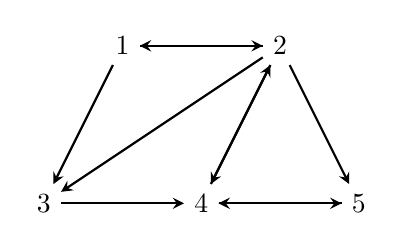
\begin{tikzpicture}[->, thick, >=stealth, node distance=2.5cm]
    \node (1) at (2,2) {1};
    \node (2) at (4,2) {2};
    \node (3) at (1,0) {3};
    \node (4) at (3,0) {4};
    \node (5) at (5,0) {5};

    \draw (1) -- (2);
    \draw (1) -- (3);
    \draw (2) -- (1);
    \draw (2) -- (3);
    \draw (2) -- (4);
    \draw (2) -- (5);
    \draw (3) -- (4);
    \draw (4) -- (2);
    \draw (4) -- (5);
    \draw (5) -- (4);
\end{tikzpicture}

2.矩阵:
$$
\begin{bmatrix}
    0 & 1 & 1 & 0 & 0\\
    1 & 0 & 1 & 1 & 1\\
    0 & 0 & 0 & 1 & 0\\
    0 & 1 & 0 & 0 & 1\\
    0 & 0 & 0 & 1 & 0
\end{bmatrix}
$$
\subsection{T12}
$$VERT = [1, 4, 7, 11]$$
$$TAIL = [1, 1, 1, 2, 2, 2, 3, 3, 3, 3, 4, 4, 4]$$
$$HEAD = [1, 2, 4, 1, 2, 4, 1, 2, 3, 4, 1, 2, 4]$$
$$NEXT = [2, 3, 0, 5, 6, 0, 8, 9, 10, 0, 12, 13, 0]$$
\section{4.7}
\subsection{T7}
(a) $\overline{R} = \{(1, 4), (2, 1), (3, 1), (3, 2), (3, 3), (4, 2), (4, 3), (4, 4)\}$\\
(b) $R \cap S = \{(1, 1), (1, 2), (2, 2), (2, 3), (2, 4), (3, 4), (4, 1)\}$\\
(c) $R \cup S = \{(1, 1), (1, 2), (1, 3), (1, 4), (2, 2), (2, 3), (2, 4), (3, 1), (3, 2), (3, 4), (4, 1), (4, 4)\}$\\
(d) $S^{-1} = \{(1, 1), (1, 3), (1, 4), (2, 1), (2, 2), (2, 3), (3, 2), (4, 1), (4, 2), (4, 3), (4, 4)\}$  
\subsection{T8}
(a) $\overline{R} = \{(a, c), (a, e), (b, a), (b, c), (b, d), (c, a), (c, c), (c, d), (c, e), (d, a), (d, b),\\
(d, e), (e, c), (e, d), (e, e)\}$\\
(b) $R \cap S = \{(a, a), (a, d), (c, b), (e, a), (e, b)\}$\\
(c) $R \cup S = \{(a, a), (a, b), (a, d), (a, e), (b, a), (b, b), (b, e), (c, b), (c, d), (d, c), (d, d),\\
(e, a), (e, b), (e, d), (e, e)\}$\\
(d) $S^{-1} = \{(a, a), (a, b), (a, e), (b, c), (b, e), (d, a), (d, c), (d, e), (e, a), (e, e)\}$
\subsection{T12}
(a) $M_{R\cap S} = 
\begin{bmatrix}
    0 & 0 & 0\\
    0 & 0 & 1\\
    0 & 0 & 0\\
    0 & 1 & 0
\end{bmatrix}$\quad
(b) $M_{R \cup S} = 
\begin{bmatrix}
    1 & 1 & 1\\
    1 & 1 & 1\\
    0 & 1 & 1\\
    1 & 1 & 1
\end{bmatrix}$\\
(c) $R^{-1} = 
\begin{bmatrix}
    0 & 0 & 0 & 1\\
    1 & 1 & 0 & 1\\
    0 & 1 & 1 & 1
\end{bmatrix}$\quad
(d) $M_{\overline{S}} = 
\begin{bmatrix}
    0 & 1 & 0\\
    0 & 1 & 0\\
    1 & 0 & 1\\
    1 & 0 & 1
\end{bmatrix}$
\subsection{T14}
$R\cap S = \{(1, 1), (1, 2), (2, 1), (2, 2), (3, 3), (4, 4), (5, 5), (6, 6)\}$\\
划分:$\{\{1, 2\}, \{3\}, \{4\}, \{5\}, \{6\}\}$。
\subsection{T19}
因为闭包运算是往集合里面添加元素的过程,相当于让关系矩阵中的部分的0变为1,但是不能把1变为0。
因此例如一个等价关系,往里面不断将0化为1,都不能使其具有非自反、非对称、反对称关系。
因此闭包的概念不适用于非自反、非对称、反对称之中。
\subsection{T20}
(a) $R \circ S = \{(a, c) | a \leq 6c\}$。因为$2 \leq 6 \times 3 = 18$,因此$(2, 3) \in R \circ S$。\\
(b) 因为$8 \geq 6 \times 1$,因此$(8, 1) \notin R \circ S$
\subsection{T23}
(a) 自反性:假设$R$, $S$是$A$上的关系,且都具有自反性。$\forall x \in A \rightarrow (x, x) \in R \land (x, x) \in S$.
所以对于$R \circ S$而言,有$\forall x \in A, (x, x) \circ (x, x) = (x, x)$。因此$R \circ S$仍为自反的。\\
反自反性:假设$R = \{(1, 2)\}, S = \{(2, 1)\}$,则$R \circ S = \{(1, 1)\}$。反自反不能保持
对称性:假设$R = \{(1, 2), (2, 1)\}, S = \{(2, 3), (3, 2)\}$,则$R \circ S = \{(1, 3)\}$,对称性不能保持。\\
反对称性:假设$R = \{(1, 2), (2, 2)\}, S = \{(2, 2), (1, 1), (2, 1)\}$,则$R \circ S = \{(1, 2), (1, 1), (2, 2), (2, 1)\}$,
反对称性不能保留
传递性:假设$R = \{(1, 2), (2, 4)\}, S = \{(2, 2), (4, 3)\}$,则$R \circ S = \{(1, 2), (2, 3)\}$,对称性不能保持。\\
(b) 自反性:根据(a)中可知,自反性质能够保留,因此$S \circ R$是$A$上的自反关系。\\
对称性:假设$R = \{(1, 1), (1, 2), (2, 1), (2, 2), (3, 3)\}, S = \{(1, 1), (2, 2), (2, 3), (3, 2), (3, 3)\}$。
所以$S \circ R = \{(1, 1), (1, 2), (1, 3), (2, 1), (2, 2), (2, 3), (3, 3), (3, 2)\}$,不满足对称性。
因此$S \circ R$不是A上的等价关系
\subsection{T24}
(a) $M_{R \circ R}= 
\begin{bmatrix}
    1 & 1 & 1 & 1 & 1\\
    1 & 1 & 1 & 1 & 0\\
    1 & 0 & 1 & 1 & 1\\
    1 & 0 & 1 & 1 & 1\\
    1 & 1 & 1 & 1 & 1
\end{bmatrix}$ \quad
(b) $M_{S \circ R} = 
\begin{bmatrix}
    1 & 1 & 1 & 1 & 1\\
    1 & 0 & 1 & 0 & 0\\
    1 & 1 & 1 & 1 & 1\\
    1 & 0 & 1 & 1 & 0\\
    1 & 1 & 1 & 1 & 1
\end{bmatrix}$\\
(c) $M_{R \circ S} = 
\begin{bmatrix}
    1 & 0 & 1 & 1 & 1\\
    1 & 0 & 1 & 1 & 1\\
    1 & 0 & 1 & 1 & 1\\
    1 & 1 & 1 & 1 & 1\\
    1 & 1 & 1 & 1 & 1
\end{bmatrix}$ \quad
(d) $M_{S \circ S} = 
\begin{bmatrix}
    1 & 1 & 1 & 1 & 1\\
    1 & 0 & 1 & 1 & 0\\
    1 & 0 & 1 & 1 & 0\\
    1 & 1 & 1 & 1 & 1\\
    1 & 0 & 0 & 1 & 1
\end{bmatrix}$
\subsection{T26}
因为$R \cap R^{-1} = S \cap S^{-1} = \varnothing$,所以
\begin{align*}
    (R \cap S) \cap (R \cap S)^{-1} &= (R \cap S) \cap (R^{-1} \cap S^{-1})\\
    &= (R \cap R^{-1}) \cap (S \cap S^{-1})\\
    &= \varnothing
\end{align*}
因此$R \cap S$是非对称的。
\begin{align*}
    (R \cup S) \cap (R \cup S)^{-1} &= (R \cup S) \cap (R^{-1} \cup S^{-1})\\
    &= ((R \cup S) \cap R^{-1}) \cup ((R \cup S) \cap S^{-1})\\
    &= R \cap R^{-1} \cup S \cap R^{-1} \cup R \cap S^{-1} \cup S \cap S^{-1}\\
    &= S \cap R^{-1} \cup R \cap S^{-1}\\
    &= S \cap R^{-1} \cup (S \cap R^{-1})^{-1}
\end{align*}
因此,如果$S \cap R^{- 1} = \varnothing$,$R \cup S$是非对称的,反之则不是。
\subsection{T27}
假设$R = \{(1, 1), (1, 2), (2, 2)\}, S = \{(1, 1), (2, 2), (2, 1)\}$。因此
$R \cup S = \{(1, 1), (1, 2), (2, 1), (2, 2)\}$是对称的,不是反对称的。\\
对于$R \cap S$,如果$\forall (a, b) ((a, b) \in  (R \cap S) \land (b, a) \in (R \cap S))$,故$(a, b) \in R \land (b, a) \in R$。
因为$R$是反对称的,因此$a = b$,故$R \cap S$是反对称的。
\subsection{T28}
对$\forall a \in A, c \in C$,有$a (S \cup T) \circ R c$
\begin{align*}
    a(S \cup T) \circ Rc &\Leftrightarrow (\exists b \in B)(a(S \cup T)b \land bRc)\\
    &\Leftrightarrow (\exists b \in B)((aSb \lor aTb) \land bRc)\\
    &\Leftrightarrow (\exists b \in B)(aSb \land bRc \lor aTb \land bRc)\\
    &\Leftrightarrow (\exists b \in B)(a S \circ R c \lor a T \circ R c)\\
    &\Leftrightarrow (a (S \circ R) \cup (T \circ R)c)
\end{align*}因此$(S \cup T)\circ R = (S \circ R) \cup (T \circ R)$
\subsection{T30}
$\forall a \in A, c \in C$,有$a T \circ R c$.
\begin{align*}
    a T \circ R c &\Rightarrow (\exists b \in B)(aTb \land bRc)\\
    &\Rightarrow (\exists b \in B)(aTb \land bSc)\\
    &\Rightarrow a T \circ S b
\end{align*}因此:$T \circ R \subseteq T \circ S$
\subsection{T31}
(a) 因为$\forall a \in A, b \in A, a(R \cap S)b \Leftrightarrow aRb \land aSb$。
因此$(a, b) \in (R \cap S) \Leftrightarrow (a, b) \in R \land (a, b) \in S$,
故$M_{R\cap S} = M_R \land M_S$\\
(b) 因为$\forall a \in A, b \in A, a(R \cup S)b \Leftrightarrow aRb \lor aSb$。
因此$(a, b) \in (R \cup S) \Leftrightarrow (a, b) \in R \lor (a, b) \in S$,
故$M_{R \cup S} = M_R \lor M_S$\\
(c) 因为$\forall a \in A, b \in A, (a, b) \in R^{-1} \Leftrightarrow (b, a) \in R$,
故$M_{R^{-1}} = (M_R)^T$\\
(d) 因为$\forall a \in A, b \in A, (a, b) \in \overline{R} \Leftrightarrow (a, b) \notin R$,
故$M_{\overline{R}} = \overline{M_R}$
\subsection{T36}
$\forall (a, b) \in R \land (a, b) \notin S$因为$R,S$都是对称的,因此$(b, a) \in R \land (b, a) \notin S$。
故$\forall (a, b) \in R \land (a, b) \notin S \Rightarrow (b, a) \in R \land (b, a) \notin S$。
因此$\forall (a, b) \in (R - S) \Rightarrow (b, a) \in (R - S)$,即$R - S$也是一个对称关系。
\subsection{T37}
(a) 充分性:$R$是对称的 $\Rightarrow R = R^{-1}$\\
$\forall (b, a) \in R \Rightarrow (a, b) \in R^{-1}$,又因为$R$是对称的,
因此$\forall (b, a) \in R \Rightarrow (a, b) \in R$。因此$R \subseteq R^{-1}$。
同理$R^{-1} \subseteq R$,因此$R = R^{-1}$。\\
必要性:$R = R^{-1} \Rightarrow R$ 是对称的\\
因为$R = R^{-1}$,$\forall (a, b) \in R \Rightarrow (a, b) \in R^{-1}$,又因为
$\forall (a, b) \in R^{-1} \Rightarrow (b, a) \in R$。因此$\forall (a, b) \in R \Rightarrow (b, a) \in R$。
故$R$是对称的。

(b) 充分性:$R$是反对称的 $\Rightarrow R \cap R^{-1} \subseteq \Delta$\\
$\forall a \in A, b \in B$,\\
当$a \neq b$时,$\forall (a, b) \in R \Rightarrow (b, a) \notin R \Rightarrow (a, b) \notin R^{-1}$。
因此$R \cap R^{-1} = \varnothing$。\\
当$a = b$时,$\forall (a, b) \in R \Rightarrow (b, a) \in R \Rightarrow (a, b) \in R^{-1}$,
因此$R \cap R^{-1} \subseteq \Delta$。\\
综上所述:$R$是反对称的 $\Rightarrow R \cap R^{-1} \subseteq \Delta$\\
必要性:$R \cap R^{-1} \subseteq \Delta \Rightarrow R$ 是反对称的\\
$\forall a \in A, b \in B$,\\
当$a \neq b$时,$\forall (a, b) \in R \Rightarrow (a, b) \notin R^{-1} \Rightarrow (b, a) \notin R$。
因此$\forall a \in A, \nexists b(b \in A \land b \neq a) \Rightarrow (a, b) \in R \land (b, a) \in R$\\
当$a = b$时,$\forall (a, b) \in R \Rightarrow (b, a) \in R \Rightarrow (a, b) \in R^{-1}$。\\
综上所述:$R \cap R^{-1} \subseteq \Delta \Rightarrow R$ 是反对称的\\
(c) 充分性:$R$是非对称的 $\Rightarrow R \cap R^{-1} = \varnothing$\\
因为$R$是非对称的,因此$\forall (a, b) \in R \Rightarrow (b, a) \notin R \Rightarrow (a, b) \notin R^{-1}$,
故$R \cap R^{-1} = \varnothing$\\
必要性:$R \cap R^{-1} = \varnothing \Rightarrow R$ 是非对称的\\
因为$R \cap R^{-1} = \varnothing$,因此$\forall (a, b) \in R \Rightarrow (a, b) \notin R^{-1} \Rightarrow (b, a) \notin R$,
因此$R$是非对称的。\\
\section{4.8}
\subsection{T8}
充分性:$a S^{\infty} b \Rightarrow R$中存在从$a$到$b$的一条路径,且该路径具有偶数条边。\\
因为$S = R^2$,因为$a S^{\infty}b \Rightarrow \exists i \geq 1 s.t. a S^i b$。
又因为$S^i = R^{2i}$,所以存在一条从$a$到$b$长度为$2i$的路径。即$a S^{\infty} b \Rightarrow R$中存在从$a$到$b$的一条路径,且该路径具有偶数条边。\\
必要性:$R$中存在从$a$到$b$的一条路径,且该路径具有偶数条边 $\Rightarrow a S^{\infty} b $\\
因为$R$中存在从$a$到$b$的一条路径,且该路径具有偶数条边。不妨设$aR^{2k}b$,因为$S = R^2$,
故$a S^k b$. 又因为$S^k \subseteq S^{\infty}$,即$a S^{\infty} b$。\\
综上所述:$a S^{\infty} b $当且仅当$ R$中存在从$a$到$b$的一条路径,且该路径具有偶数条边。
\subsection{T10}
$M_R = 
\begin{bmatrix}
    1 & 1 & 0 & 0\\
    1 & 0 & 0 & 0\\
    0 & 0 & 0 & 0\\
    0 & 0 & 1 & 0
\end{bmatrix},\quad 
M_{R^2} = 
\begin{bmatrix}
    1 & 1 & 0 & 0\\
    1 & 0 & 0 & 0\\
    0 & 0 & 0 & 0\\
    0 & 0 & 1 & 0
\end{bmatrix} = M_R$.\\
因此$M_{t(R)} = 
\begin{bmatrix}
    1 & 1 & 0 & 0\\
    1 & 0 & 0 & 0\\
    0 & 0 & 0 & 0\\
    0 & 0 & 1 & 0
\end{bmatrix}$
\subsection{T12}
$M_R = 
\begin{bmatrix}
    0 & 0 & 0 & 1\\
    1 & 0 & 0 & 1\\
    0 & 1 & 0 & 1\\
    0 & 0 & 1 & 0
\end{bmatrix}, \quad
M_{R^2} = 
\begin{bmatrix}
    0 & 0 & 0 & 1\\
    1 & 0 & 0 & 1\\
    1 & 1 & 0 & 1\\
    0 & 0 & 1 & 0
\end{bmatrix}, \quad
M_{R^3} = 
\begin{bmatrix}
    0 & 0 & 0 & 1\\
    1 & 0 & 0 & 1\\
    1 & 1 & 0 & 1\\
    1 & 1 & 1 & 1
\end{bmatrix},$\\
$M_{R^4} = 
\begin{bmatrix}
    1 & 0 & 1 & 1\\
    1 & 0 & 1 & 1\\
    1 & 1 & 1 & 1\\
    0 & 1 & 1 & 1
\end{bmatrix}$
因此:
$M_{t(R)} = 
\begin{bmatrix}
    1 & 0 & 1 & 1\\
    1 & 0 & 1 & 1\\
    1 & 1 & 1 & 1\\
    0 & 1 & 1 & 1
\end{bmatrix}$
\subsection{T14}
$M_R = 
\begin{bmatrix}
    0 & 0 & 0 & 0\\
    1 & 1 & 1 & 0\\
    0 & 1 & 1 & 0\\
    0 & 1 & 0 & 0
\end{bmatrix}$\\
求$M_s{(R)}$的传递闭包关系矩阵:
$M_{s(R)} = 
\begin{bmatrix}
    0 & 1 & 0 & 0\\
    1 & 1 & 1 & 1\\
    0 & 1 & 1 & 0\\
    0 & 1 & 0 & 0
\end{bmatrix}$,
$M_{s(R)^2} = 
\begin{bmatrix}
    1 & 1 & 1 & 1\\
    1 & 1 & 1 & 1\\
    1 & 1 & 1 & 1\\
    1 & 1 & 1 & 1
\end{bmatrix}$
故:$M_{t(s(R))} = 
\begin{bmatrix}
    1 & 1 & 1 & 1\\
    1 & 1 & 1 & 1\\
    1 & 1 & 1 & 1\\
    1 & 1 & 1 & 1
\end{bmatrix}$\\
求$M_{t(R)}$的对称闭包关系矩阵:
$M_{R^2} = 
\begin{bmatrix}
    0 & 0 & 0 & 0\\
    1 & 1 & 1 & 0\\
    1 & 1 & 1 & 0\\
    1 & 1 & 1 & 0
\end{bmatrix}, \quad$
$M_{R^3} = M_{R^2}$.
因此$M_{s(t(R))} = 
\begin{bmatrix}
    0 & 1 & 1 & 1\\
    1 & 1 & 1 & 1\\
    1 & 1 & 1 & 1\\
    1 & 1 & 1 & 0
\end{bmatrix}$
因此:$R_t$的对称闭包和$R_s$的传递闭包不具有相同的关系
\subsection{T18}
$A / R = \{\{1\}, \{2, 3\}, \{4 ,5\}\}, A / S = \{\{1, 2\}, \{3\}, \{4, 5\}\}$.\\
$A / (R \cup S)^\infty = \{\{1, 2, 3\}, \{4, 5\}\}$
\subsection{T20}
因为19题的前提条件是两个关系本身是等价关系,不具有普遍性。而Warshall算法不需要这个前提条件。
\subsection{T23}
使用了直接证明法。先假设$\forall S, (R \subseteq S)$,后续利用$S$的传递性,说明$S^{\infty} \subseteq S$,
又因为满足公式$S^{\infty} = \bigcup_{n = 1}^{\infty}S^n \subseteq S$,结合$R \subseteq S$,推出$R^{\infty} \subseteq
S^{\infty} \subseteq S$。从而证明是传递关系中最小的。
\subsection{T24}
使用了构造性证明法。考虑了路径中可能成环,把成环的部分删去,留下顶点各异的部分。因为顶点数不可能超过n,
因此路径的长度也至多是n。由此证明计算$R^{\infty}$并不需要计算比$n$次幂大的$R$的幂。
\subsection{T25}
设包含$R$的最小等价关系为$S$.\\
$S$满足自反性:$\forall x \in A, (x, x) \in S$。\\
$S$满足对称性且$R \subseteq s$:$\forall a \in A, b \in A \land |a| \leq |b| \Rightarrow (a, b) \in R \Rightarrow (a, b) \in S$,
因为$S$满足对称性,所以$|a| \geq |b| \Rightarrow (a, b)\in S \Rightarrow a \in A, b \in A a \neq b \Rightarrow (a, b) \in S$。\\
综上所述,$\forall a \in A, b \in A.$当$a = b, (a, b) \in S$。当$a \neq b, (a, b) \in S$。
因此,$\forall a \in A, b \in A \Rightarrow (a, b) \in S$即$S = A \times A = \mathbf{R} \times \mathbf{R}$。 
\end{document}